
\section{Background \& Problem}

All Open Container Initiative compliant containers, including Kubernetes,
enforce CPU reservations using \cgroups{}' weight interface~\cite{oci-cgroups,
docker-docs-cgroups, container-isolation-article}, as do VM frameworks,
including Firecracker and
libvirt~\cite{firecracker-cgroups,afaas,libvirt-cgroups}. 

\begin{figure}[t]
    \centering
    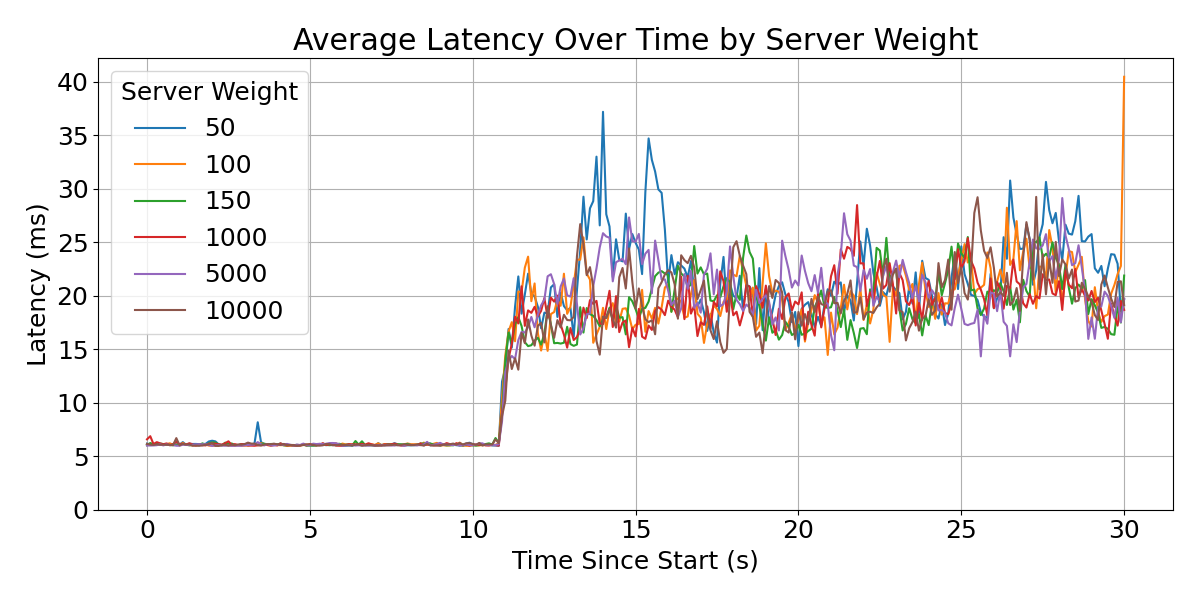
\includegraphics[width=\columnwidth]{graphs/srv-bg-weight-cmp-low.png}
    \caption{ the weight of the server has little impact on how much the
    weight 1 BE task interferes }\label{fig:srv-bg-weight-cmp}
\end{figure}


A simplified experiment shows \cgroups{} weights are unable to enforce
reservations. We run a simple CPU-bound server sharing four cores with an image
resize job, each in their own group. \cgroups{} supports weights in the range of
[1,10000]. \autoref{fig:srv-bg-weight-cmp} shows that running the server with
different weights has no effect on the latency impact of the BE.

\begin{figure}[t]
    \centering
    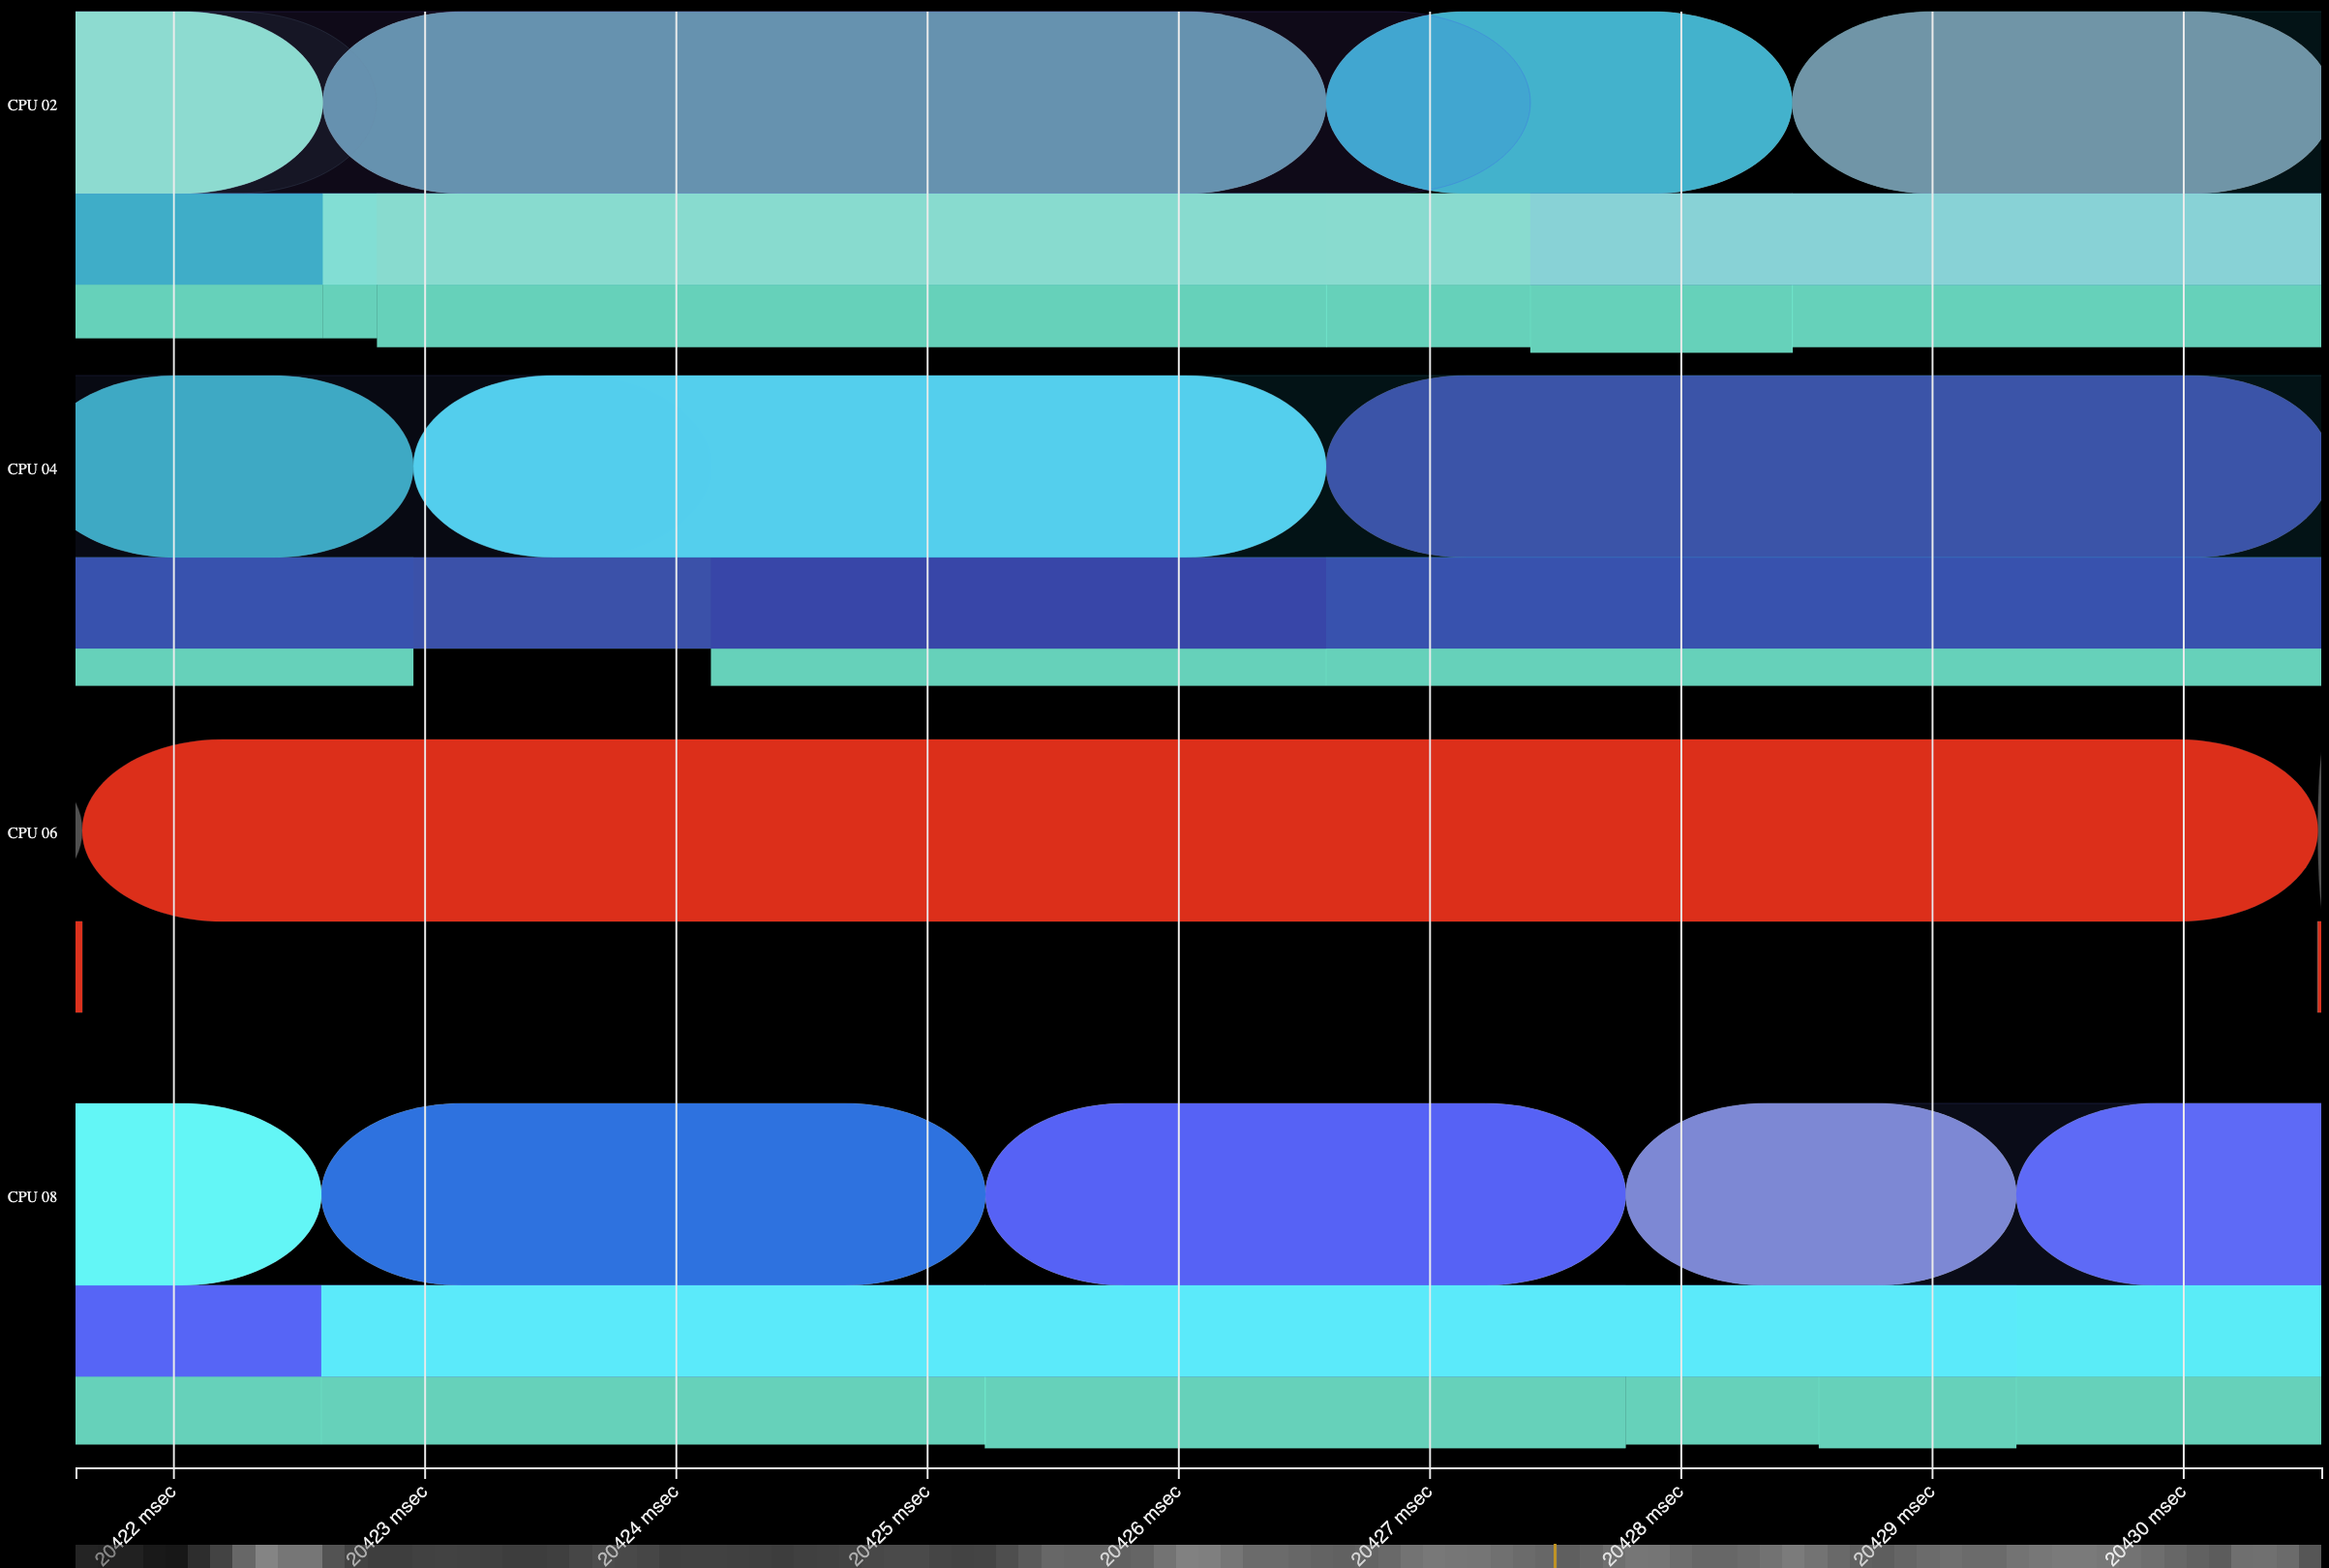
\includegraphics[width=\columnwidth]{graphs/schedviz-problem.png}
    \caption{Core 6 runs an image resize process, unaware that the other cores
    have queued server threads}\label{fig:schedviz-problem}
\end{figure}

This latency impact happens because the BE occasionally runs uncontended on one
core, while another has queued server threads. \autoref{fig:schedviz-problem}
shows this happening in the trace: on core 6, the red BE thread runs for 10ms,
while server threads, in shades of blue, are queued on the other cores.

This happens because weights are only enforced within per-CPU runqueues. Load
balancing eventually remedies imblances, but runs less frequently than
scheduling does. For workloads with request processing times in the millisecond
range, waiting for the load balancer influences final processing times.

In order to globally enforce weights, each scheduling decision would require a
search of all runqueues for potentially higher-weight processes, which is too
costly. 




